\documentclass[a4paper,10pt]{article}
\def\chapno{1}
\usepackage{lmodern}

% (2) specify encoding
\usepackage[T1]{fontenc}

% (3) load symbol definitions
\usepackage{graphicx}
%\usepackage{textcomp}
\usepackage{hyperref}
\usepackage[utf8]{inputenc}
\usepackage[english]{babel}
\usepackage[usenames, dvipsnames]{color}
\usepackage{textcomp}
\def\'{\textquotesingle}
\def\tq{\textquotesingle}
\def\blue{\textcolor{blue}}
\def\green{\textcolor{Purple}}
%\def\green{\textcolor{ForestGreen}}
\def\lpv{lp\_var}
%\include{diagxy}
%opening
\title{LIPGLOSS Notes}
%\newline Course Information and Policies}
\author{Pieter Mostert}%\fontsize{\Large}{}Course Information and Policies}}
%\date{}
\begin{document}

\maketitle
\def\thefootnote{\fnsymbol{footnote}}\setcounter{footnote}{1}
%\setcounter{prob}{33}\fontsize{\Large}{}
\section{Introduction}
LIPGLOSS is a collection of Python scripts designed to construct ceramic recipes that satisfy a number of constraints. In particular, it allows users to construct recipes with a given oxide composition, when possible.

It employs a linear programming algorithm to calculate bounds on oxides and ingredients, hence its full name: \textit{LInear Programming GLaze Oxide Software System}. Since that's a terrible name, it\'s better to just stick with the acronym LIPGLOSS.

The plan is that LIPGLOSS will eventually be released as a stand-alone app that users can customize with their own ingredients and restrictions. This will be designed to import and export recipes from \href{https://glazy.org}{Glazy}, as well as other glaze calculation software; alternatively, part of the code could be incorporated within Glazy.

\section{Using LIPGLOSS}

Currently, to use LIPGLOSS, you need to instal \href{https://www.python.org/downloads/}{Python 3}, the linear programming API \href{https://github.com/coin-or/pulp}{PuLP}, and the \href{https://www.gnu.org/software/glpk/}{GLPK} library\footnote{If installing the GLPK library is a problem, comment out `solver = GLPK()' and uncomment `solver = PULP\_CBC\_CMD()' in pulp2dim.py. This will result in the COIN-OR \href{https://projects.coin-or.org/Cbc}{Cbc} solver being used, which comes with PuLP. Note, however, that it is released under the \href{https://en.wikipedia.org/wiki/Eclipse_Public_License}{Eclipse Public Licence}, which is \href{https://eclipse.org/legal/eplfaq.php}{incompatible with the GPL}.} (and possibly the \href{https://wiki.python.org/moin/TkInter}{tkinter} Python package). Running the GUI.py script opens the graphical user interface. 

When the gui opens, you'll be presented with a window that shows a list of ingredients and `other restrictions' in the panel on the left. Some of these will have already been selected by default, but you can add or remove items by clicking on the buttons.

In the panel on the right, the selected ingredients and other restrictions will be shown, as well as any oxides that appear in the selected ingredients. The two columns on the left, which contain values in blue, are for entering the desired lower and upper bounds on the oxide, ingredient, or other restriction. Bounds on oxides can be expressed as UMF, percent weight or percent mole by selecting the appropriate radio button above. 

When you click the `Calculate restrictions' button, the two columns on the right will be filled with lower and upper bounds for each oxide, ingredient, or other restriction, printed in red (assuming there is at least one recipe that satifies the bounds; otherwise, an error message will appear). These are lower and upper bounds for the corresponding item among all possible recipes using the ingredients selected that satisfy the bounds you've imposed. Naturally, the bounds on the right are at least as restrictive as the bounds on the left.

You can now progressively strengthen the bounds on the left, based on the calculated bounds. This may be as simple as unselecting an ingredient whose calculated lower bound is zero. Given a single oxide, ingredient, or other restriction, you can narrow it's range to any interval that overlaps the calculated interval, and be guaranteed that the problem still has a solution\footnote{Actually, this is a lie, since the calculated bounds are rounded to a certain number of decimal places, so, for example, setting the upper bound equal to the calculated lower bound won't work if the calculated lower bound has been rounded down.}. However, it's important to note that if you restrict the bounds for two or more items simultaneously, a solution is not guaranteed even if the restricted intervals both overlap their respective calculated intervals\footnote{For example, if only two ingredients are selected and no restrictions are imposed, the bounds on the percentages of these ingredients will be 0 and 100. If you then impose the bounds 0 to 40 on both these ingredient percentages, there will be no solution, simply because the sum of the ingredient percentages must add up to 100.}.

If you want to restrict the bounds for two variables simultaneously, you have the option of plotting the set of possible values of those two variables. That is to say, for each point in the region shown, there is at least one recipe where the variables take on the $x$ and $y$ values of the point, and which satisfies all the constraints\footnote{If you take the example in the previous footnote, the region corresponding to the two ingredient percentages will be a straight line from $(0,100)$ to $(100,0)$. Typically, the regions that arise will be two dimensional, and will always have boundaries that are either straight lines or sections of hyperbolas.}. The $x$ and $y$ variables to plot can be selected by clicking on the left and right hand labels in the right hand panel, respectively. An asterisk should appear next to the label when you click on it. At the moment it's only possible to compare variables of the same type, so you can't plot the percentage of an ingredient together with the mole percentage of an oxide, or the UMF of an oxide together with the weight percentage of an oxide.

A collection of ingredient and other restrictions with lower and upper bounds will be referred to as a bounded recipe. Bounded recipes can be saved, or saved as new bounded recipes (at the moment, their names are determined automatically). If you start with the default bounds and narrow them down to a recipe - i.e. all upper and lower bounds are effectively the same - you should save this as a new bounded recipe, otherwise you'll have to undo all your restrictions when you start working on a new problem. Saved bounded recipes can be opened through the File menu.

LIPGLOSS will come pre-installed with common types of ingredients, but most of these should be updated to reflect the analyses of the ingredients in your studio. To do this, click Options $>$ Edit Ingredients to open the ingredient editor.

\section{Code Structure}
In an attempt to make things clearer, any text below that is used as code will be printed in blue. File names will be printed in purple.

As noted before, the \green{GUI.py} file launches the gui. The following diagram shows the import relations between the modules.
%\green{GUI.py} imports the modules \green{vert\_scrolled\_frame.py}, \green{polyplot.py},
%\green{pulp2dim.py}, \green{restriction\_class.py} and \green{recipe\_class.py} (along with a number of built-in Python modules). The \green{recipe\_class.py} module imports \green{restriction\_class.py} and \green{pulp2dim.py}, while \green{restriction\_class.py} imports \green{gui\_basic\_framework.py} and \green{pretty\_names.py}, and \green{gui\_basic\_framework.py} imports \green{vert\_scrolled\_frame.py}.

%Graph generated by www.webgraphviz.com
%digraph module_dependencies {
%	ratio = fill;
%	node [style=filled];
%	vert_scrolled_frame -> gui_basic_framework;
%	gui_basic_framework -> restriction_class;
%	restriction_class -> recipe_class;
%	pretty_names -> restriction_class ;
%	pulp2dim -> recipe_class ;
%	polyplot -> GUI 
%	recipe_class -> GUI;
%}

\begin{figure}[ht!]
\centering
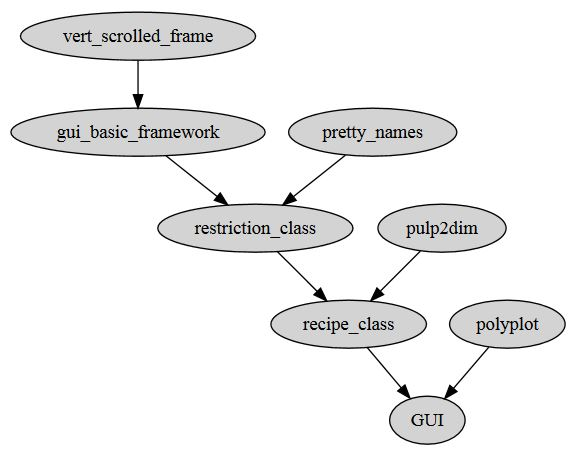
\includegraphics[width=90mm]{Module_dependencies.jpg}
\caption{Module dependencies \label{dep}}
\end{figure}

The files \green{ingredientfile.py} and \green{oxidefile.py} are usually not used, and can be omitted from any stable releases. See section 0 in \green{GUI.py} for when they are needed.

The following classes are defined: \blue{Oxide}, \blue{Ingredient}, \blue{Other}, \blue{Restriction} (see \green{restriction\_class.py}) and \blue{Recipe} (see \green{recipe\_class.py}). To keep track of the instances of these classes, we use the dictionaries \blue{oxide\_dict}, \blue{ingredient\_dict}, \blue{other\_dict}, \blue{restr\_dir}, and \blue{recipe\_dict}. The keys for the \blue{ingredient\_dict}, \newline \blue{other\_dict}, and \blue{recipe\_dict} dictionaries are strings of non-negative integers. The keys for \blue{oxide\_dict} are strings of the form \blue{\'SiO2\'}, \blue{\'Al2O3\'}, etc.  There are five types of \blue{Restriction} instances, so keys are of five different types:
\begin{itemize}
\item \blue{\'umf\_\'+ox}, \blue{\'mass\_perc\_\'+ox}, and \blue{\'mole\_perc\_\'+ox}, for each key \blue{ox} in \blue{oxide\_dict},
\item \blue{\'ingredient\_\'+k} for each key \blue{k} in \blue{ingredient\_dict}, 
\item \blue{\'other\_\'+k} for each key \blue{k} in \blue{other\_dict}. 
\end{itemize}

We could easily do without the \blue{Oxide} class, but I've introduced it so that if (in some future version of the program) we decide to allow users to assign attributes to oxides, then this can be done in the same way as for ingredients. See the `To do' list.

\subsection{Setting up the linear programming problem}
The code relating to the computation of the bounds is mostly found in \newline
\green{recipe\_class.py}, although parts of the linear programming problem are set up in \green{GUI.py}. To set up the LP problem, we define the following variables / families of variables:
\begin{itemize}
\item \blue{\lpv[\'mass\_\'+ox]}, for each key \blue{ox} in \blue{oxide\_dict}, representing the mass (in grams) of that oxide in a batch.
\item \blue{\lpv[\'mole\_\'+ox]}, for each key \blue{ox} in \blue{oxide\_dict}, representing the number (in moles) of that oxide in a batch.
\item \blue{\lpv[\'ingredient\_\'+k]} for each key \blue{k} in \blue{ingredient\_dict}, representing the mass (in grams) of the ingredient in a batch.
\item \blue{\lpv[\'other\_\'+k]} for each key \blue{k} in \blue{other\_dict}. 
\item \blue{\lpv[\'ingredient\_total\']}, representing the total mass (in grams) of all ingredients in the batch.
\item \blue{\lpv[\'fluxes\_total\']}, representing the total number (in moles) of all flux oxides in the batch.
\item \blue{\lpv[\'ox\_mass\_total\']}, representing the total mass (in grams) of all oxides in the batch.
\item \blue{\lpv[\'ox\_mole\_total\']}, representing the total number (in moles) of all oxides in the batch.
\end{itemize}
%
These variables are related as follows:
%
\begin{itemize}
\item For each oxide \blue{ox}, 
$$\textnormal{\blue{\lpv[\'mass\_\'+ox]}} = M\times \blue{\textnormal{\lpv[\'mole\_\'+ox]}},$$
where $M$ is the molar mass of that oxide.
\item For each oxide \blue{ox}, 
$$\textnormal{\blue{\lpv[\'mass\_\'+ox]}} = \sum_{\textnormal{\blue{k}}\in\mathcal{I}} \frac{P_{\textnormal{\blue{k},\blue{ox}}}}{100} \times \textnormal{\blue{\lpv[\'ingredient\_\'+k]}},$$ 
where $\mathcal{I}$ is the set of all ingredients, and $P_{\blue{\textnormal{k}},\blue{\textnormal{ox}}}$ is the percent mass of \blue{ox} in ingredient \blue{k}.
\item For each index \blue{k} in \blue{other\_dict}, 
$$\textnormal{\blue{\lpv[\'other\_\'+k]}} = \begin{array}{l}\textnormal{a linear combination of the variables}\\
\textnormal{corresponding to ingredients and oxides}
\end{array}$$ 
\item $$\textnormal{\blue{\lpv[\'ingredient\_total\']} = $\sum_{\textnormal{\blue{k}}\in\mathcal{I}}$ \blue{\lpv[\'ingredient\_\'+k]}}$$, 
\item $$\textnormal{\blue{\lpv[\'fluxes\_total\']}} = \sum_{\blue{\textnormal{ox}}\in \mathcal{F}} \textnormal{\blue{\lpv[\'oxide\_mol\_\'+ox]}},$$ 
where $\mathcal{F}$ is the set of all fluxes, 
\item $$\textnormal{\blue{\lpv[\'ox\_mass\_total\']}} = \sum_{\blue{\textnormal{ox}}\in \mathcal{O}} \textnormal{\blue{\lpv[\'mass\_\'+ox]}},$$ where $\mathcal{O}$ is the set of all oxides,  
\item $$\textnormal{\blue{\lpv[\'ox\_mole\_total\']}} = \sum_{\blue{\textnormal{ox}}\in \mathcal{O}} \textnormal{\blue{\lpv[\'mole\_\'+ox]}}.$$
\end{itemize}
%These relations always hold (unless the ingredients are changed). 

Note that the quantities we'd like to optimize are not the basic variables \blue{\lpv[}\ldots\blue{]}, but certain \emph{ratios} of these variables. For example, the UMF value of an oxide \blue{ox} is $$\frac{\textnormal{\blue{\lpv[\'mole\'+ox]}}}{\textnormal{\blue{\lpv[\'fluxes\_total\']}}},$$ 
while the percentage of an ingredient with index \blue{k} is $$100\times\frac{\textnormal{\blue{\lpv[\'ingredient\'+k]}}}{\textnormal{\blue{\lpv[\'ingredient\_total\']}}}.$$

In general, given a restriction \blue{res}, the associated quantity we want to optimize is of the form \blue{\lpv[}numerator\blue{]}/\blue{res.normalization} where `numerator' and \blue{res.normalization} are defined below:

\begin{flushleft}
\begin{tabular}{|p{0.22\textwidth}|p{0.2\textwidth}| p{0.41\textwidth}| } \hline
 restriction                   & numerator                     & \blue{res.normalization} \\ \hline
 \blue{\tq umf\_\tq+ox}        & \blue{\tq mole\_\tq+ox} & \blue{\lpv[\tq fluxes\_total\tq]} \\ \hline
 \blue{\tq mass\_perc\_\tq+ox} & \blue{\tq mass\_\tq+ox} & $0.01\times$\blue{\lpv[\tq oxide\_mass\_total\tq]}  \\ \hline
 \blue{\tq mole\_perc\_\tq+ox} & \blue{\tq mole\_\tq+ox} & $0.01\times$\blue{\lpv[\tq oxide\_mole\_total\tq]}  \\ \hline
 \blue{\tq ingredient\_\tq+k}  & \blue{\tq ingredient\_\tq+k} & $0.01\times$\blue{\lpv[\tq ingredients\_total\tq]}  \\ \hline
 \blue{\tq other\_\tq+k}       & \blue{\tq other\_\tq+k} &  Custom \\ \hline
\end{tabular}
\end{flushleft}

When \blue{recipe.calc\_restrictions(}\ldots\blue{)} is run, for each restriction \blue{res}, we impose the constraints
$$\textnormal{\blue{\lpv[}numerator\blue{]}< $U\times$ \blue{res.normalization} }$$
and 
$$\textnormal{\blue{\lpv[}numerator\blue{]}> $L\times$ \blue{res.normalization} },$$
where $U$ and $L$ are the upper and lower bounds imposed by the user respectively.

To maximize or minimize the variable associated with a restriction \blue{res}, we set the `normalization' constraint \blue{res.normalization}=1, and maximize or minimize \blue{\lpv[}numerator\blue{]}. 

\emph{Remark}: We could eliminate all the variables other than the ones corresponding to the selected ingredients before we hand the problem over to the solver. It remains to be seen by how much this would speed up the computation time. Since the computation time for typical problems is currently only about 2 seconds, implementing this is not a high priority.

\subsection{Storing user-defined data}

To save data entered by the user, I\'ve chosen to use the \href{https://docs.python.org/3.6/library/shelve.html}{shelve} module. There may be better ways to do this. This results in several data files: \green{IngredientShelf.dat}, \green{OtherShelf.dat}, \green{OxideShelf.dat}, \green{RecipeShelf.dat} (these all have associated bak and dir files). 

At the moment, we could do without the \green{OxideShelf} files, since there's no way for the user to modify any data related to the oxides, but it may be possible in future versions.

\section{Known bugs}
\begin{itemize}
\item If you delete an ingredient using the ingredient editor, it will only be deleted from the current recipe (assuming it\'s one of the ingredients in the recipe). When you attempt to open a recipe that contains the deleted ingredient, you'll get an error (unless you've subsequently added a new ingredient which happens to have the same index).
\item If you edit the oxide composition of an ingredient that has been selected, the list of oxides shown doesn't change to reflect this.
\item On my computer, the PuLP API causes a window to open and close each time a linear function is optimized, resulting in a delay of around 10 seconds, even though the actual calculation usually takes under 2 seconds. There may be a fix for this, but I haven't been able to implement it.
\end{itemize}

\section{To do}
\begin{itemize}
\item Fix bugs above.
\item For the 2d graphing, have a button to the right of the restriction panel that when clicked on, opens a panel with instructions on how to select the two variables, as well as a button that calculates only the region corresponding to two variables, not all the other lower and upper bounds (Before updating the restrictions, you may want to compare several pairs of variables. In this case there's no need to recalculate all the other bounds). Include labels on the axes when the region is calculated, and make sure the numbers along the axes don't overlap. 
\item Implement the ability to plot the feasible region corresponding to any two restrictions.
\item Clicking Options $>$ Edit restriction settings, should open a window that allows you to set default lower and upper bounds for each oxide, ingredient and other restriction.
\item Allow users to define custom `other restrictions'. Users would need to specify an objective function, and a normalization.
\item Implement the ability to add other attributes to ingredients, using the restriction editor. Each other attribute will be assigned a variable, and an `other restriction' corresponding to that attribute will automatically be added. For example, an other attribute could be the percentage of an ingredient having particle diameters between two bounds.
\item Fix the headings when scrolling down in the ingredient editor. Add a horizontal scrollbar, and fix the ingredient names when scrolling sideways.
\item Allow users to name bounded recipes.
\item Import recipes (or oxide compositions of recipes) from external software, and automatically generate a recipe problem where the oxides are constrained to have the same composition as the imported recipe.
\item Convert recipe bounds to actual recipes, and export these to external software. This should only be used when the upper and lower bounds on all ingredients are sufficiently close together.
\item Include an `about box'. 
\end{itemize}
\end{document}